\documentclass[10pt]{article}

\usepackage[document]{ragged2e}

% for pdflatex
\usepackage[utf8]{inputenc}
% for hyperlink
\usepackage{hyperref}
\hypersetup{
    colorlinks=true,
    linkcolor=blue,
    filecolor=magenta,
    urlcolor=cyan,
}
% for table spanning multiples pages
\usepackage{longtable}
% for custom enum
\usepackage{enumitem}
% for removing alinea begin of paragraph
\usepackage{parskip}
\usepackage{array, xcolor, graphicx}
\usepackage[a4paper, margin=1cm]{geometry}
\title{\bfseries{\huge{Ingénieur Blockchain \& DevOps}}\\[0.75cm] \Large{5 années d'expérience dans la blockchain et les cryptoactifs}}
% no author
\author{\bfseries\Huge \vspace{-4ex}}
% no date
\date{}
% custom for column style
\definecolor{lightgray}{gray}{0.8}
% custom for column type
\newcolumntype{L}{p{0.2\textwidth}}
% custom for column type
\newcolumntype{R}{p{0.75\textwidth}}
% custom for column type
\newcommand\VRule{\color{lightgray}\vrule width 2pt}
% for bullet point outside of list
\newcommand{\tabitem}{~~\llap{$\rightarrow$}~~}
\pagestyle{empty}
\begin{document}

\begin{minipage}[t]{0.80\textwidth}
\textbf{\Large{Mohamed Amine LEGHERABA}}\\
\vspace{4ex}27 ans\\
92 bis rue Rouget de Lisle, Bezons, France\\
\href{tel:0630829000}{06 30 82 90 00}\\
\href{mailto:mlegheraba@protonmail.com}{mlegheraba@protonmail.com}\\
\href{https://github.com/MohamedLEGH}{github.com/MohamedLEGH}\\
\vspace{5ex}{\bf Français}: langue maternelle \\
{\bf Anglais}: bon niveau (TOIEC: 935) \\
\end{minipage}
\begin{minipage}[t]{0.20\textwidth}
\vspace{-3ex}
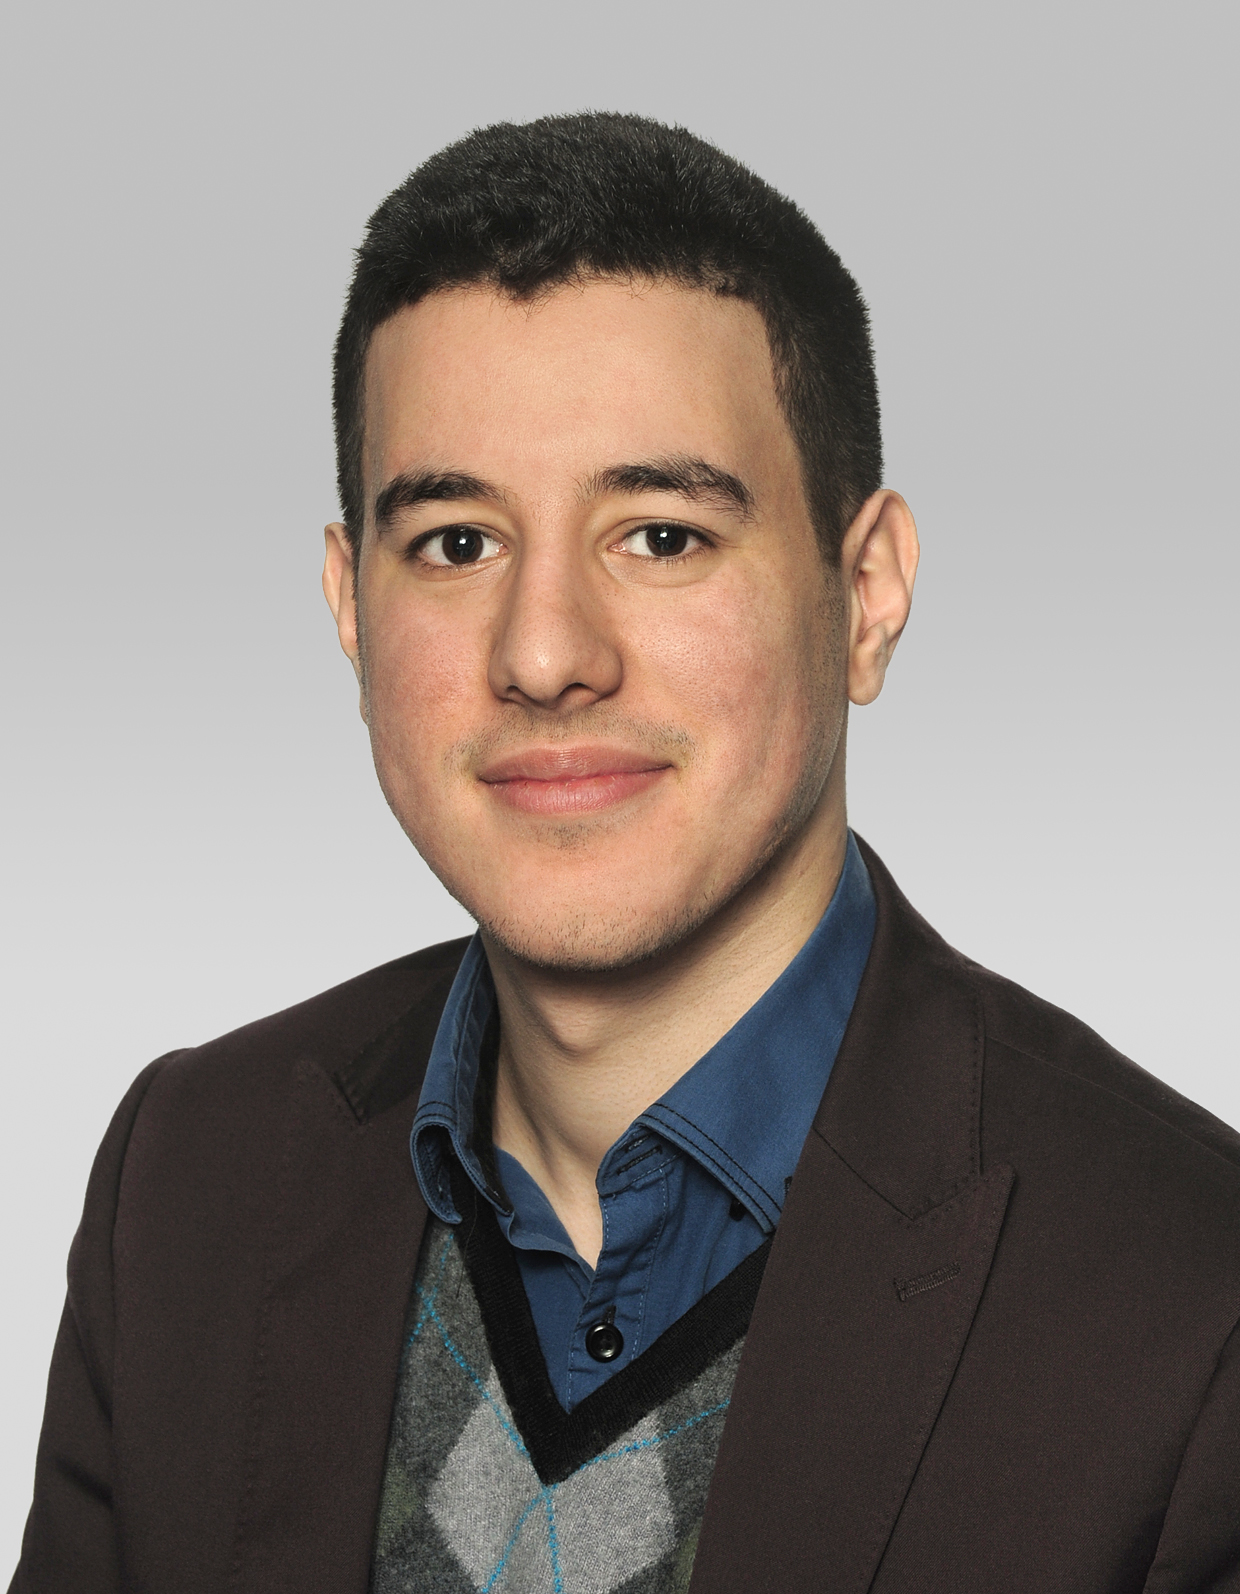
\includegraphics[width=4cm]{figures/Legheraba-Mohamed.jpg}
\end{minipage}
% to make maketitle work without begin of page
{\let\newpage\relax\maketitle}
% to remove page number
\thispagestyle{empty}

\vspace{-10ex}

\section*{Formation}

\vspace{2ex}

\begin{tabular}{L!{\VRule}R}
\textbf{\textit{2015--2018}} \hspace{1.5ex} 
\includegraphics[width=1.4cm]{figures/Logo_Reseau_Polytech.png} & \textbf{Diplôme d'Ingénieur, Polytech Sorbonne}, spécialité \textit{Mathématiques Appliquées et Informatique Numérique}: Statistiques, Équations différentielles, Programmation, Structures de données, Parallélisme.\\[0.75cm]
\textbf{\textit{2017 (Hiver)}} \hspace{.5ex} 
\includegraphics[width=.85cm]{figures/TU.png} & \textbf{Semestre Erasmus à TU Delft}, Pays-Bas: Théorie des graphes, Cryptographie, Blockchain, Cloud Computing, Visualisation de données.\\[0.75cm]
\textbf{\textit{2013--2015}} \hspace{3ex} 
\includegraphics[width=.85cm]{figures/PEIP_logo.png} & \textbf{Polytech Sorbonne}, \textit{PeiP} (Parcours des écoles d'ingénieurs Polytech): Maths, Informatique, Physique, Chimie, Mécanique.\\[0.75cm]
\textbf{\textit{2013}} & \textbf{Baccalauréat S}, mention Bien. Lycée Chaptal.\\
\end{tabular}

\vspace{2ex}

\section*{Expérience Professionnelle}

\vspace{2ex}

\begin{longtable}{L!{\VRule}R}
\textbf{\textit{Depuis Juin 2021}}& 
\includegraphics[width=1.5cm]{figures/Deloitte.png} \hspace{0.2cm} {\bf Ingénieur Sénior Blockchain \& DevOps, Deloitte.} \\[0.25cm]

& \tabitem \small{\textbf{Missions d'appui aux équipes d'audit financier} (Audit des transactions sur la blockchain, revue du contrôle interne et des procédures de conservation)}

\\[0.20cm]
& \tabitem \small{\textbf{Missions d'audit technique} (Audit de smart contracts et d'application blockchain, revue de l'architecture)}

\\[0.20cm]
& \tabitem \small{\textbf{Missions de conseil} (Appui aux équipes blockchain des clients sur la gestion de projet blockchain et la réalisation technique des applications)}

\\[0.20cm]
& \tabitem \small{\textbf{Missions de formations} (Formations auprès des clients - banque et industrie - sur la blockchain, les crypto-actifs, les NFT et le métavers)}

\\[0.20cm]
& \tabitem \small{\textbf{Rédaction d'articles} (\href{https://www2.deloitte.com/fr/fr/pages/audit/articles/univers-metavers.html}{Article sur les NFT et le métavers}, \href{https://www2.deloitte.com/content/dam/Deloitte/fr/Documents/financial-services/Publications/future-of-money-banking.pdf}{étude sur la DeFi et les CBDC}, baromètre sur l'impact carbone de la blockchain)}


\\[0.20cm]
& \tabitem \small{\textbf{Coordination} (Coordination en France avec les équipes conseil et juridique, \& avec les équipes à l'international)}

\\[0.20cm]
& \tabitem \small{\textbf{Projet Fondation Deloitte} (Mise en place d'un \href{https://blog.deloitte.fr/acculturation-tech-blockchain-une-priorite-pour-les-nouvelles-generations/}{atelier} de découverte du sujet de la blockchain et des NFT pour une classe de collégiens de Sarcelles, en partenariat avec la Fondation Deloitte et avec NomadicLabs)}

\\[0.20cm]
\textbf{\textit{Avril 2019 - Juin 2021}}& 
\includegraphics[width=2cm]{figures/SIA_logo.png} \hspace{0.2cm} {\bf Ingénieur Blockchain \& DevOps, Sia Partners.} \\[0.25cm]

& \tabitem \small{\textbf{Experimentations MNBC à la Banque de France} (Membre du pôle blockchain en tant qu'expert technique, cadrage technique d'une expérimentation, support technique pour 2 autres expérimentations, formation des autres membres de l'équipe sur la Blockchain et la méthodologie DevOps, implémentation des pipelines CI/CD)}

\\[0.20cm]
& \tabitem \small{\textbf{Suivi des limites de trading à l'aide d'un réseau blockchain pour un fonds d'investissement} \it{Mission que j'ai obtenu moi-même grâce à mon réseau et que j'ai accompli de bout en bout}}

\\[0.20cm]
& \tabitem \small{\textbf{Création d'une application de paiement mobile en cryptomonnaies pour un distributeur français}}

\\[0.20cm]
& \tabitem \small{\textbf{Projet Heka: \href{https://heka.sia-partners.com/fr}{Usine logicielle} pour les applications Data Science} (développement des microservices en Python et en React, déploiement continu sur l'infrastructure Kubernetes, ...)}

\\[0.20cm]
& \tabitem \small{\textbf{Veille R\&D sur la blockchain, les cryptomonnaies et les systèmes distribués} (étude des réseaux blockchain Liquid, Libra et TON, des technologies Lightning Network, HTLC Atomic Swap, Zero-knowledge proofs, Raft protocol, Taproot et Multi-Party Computation, ...)}

\\[0.20cm]
& \tabitem \small{\textbf{Rédaction d'articles} (\href{https://www.sia-partners.com/fr/actualites-et-publications/de-nos-experts/la-blockchain-catalyseur-de-la-decentralisation-et-de-la}{\textit{Blockchain \& 5G}}, \href{https://www.sia-partners.com/fr/actualites-et-publications/de-nos-experts/entretien-avec-pierre-noizat-bitcoin-et-cryptomonnaies-0}{\textit{Interview de Pierre Noizat}}, ...)}

\\[0.20cm]
& \tabitem \small{\textbf{Enseignement \textit{Programmer une blockchain}} (\href{https://github.com/MohamedLEGH/tutoriel-blockchain-creation-bootstrap}{Polytech Sorbonne}, \href{https://github.com/MohamedLEGH/tutoriel-blockchain-MinesBootstrap}{Mines St Etienne}, ...)}

\\[0.20cm]
\textbf{\textit{Mars--Septembre 2018}}& 
\includegraphics[width=1.5cm]{figures/ofi-am.png} \hspace{0.2cm} {\bf Stagiaire veille R\&D, Département Développement, OFI AM}.\\

\\[0.20cm]
\textbf{\textit{2017}}& {\bf Développement pour plusieurs ICO, dont 2 qui ont levé plus de 5M\$}.\\

\end{longtable}

\vspace{2ex}

\section*{Compétences Techniques}

\vspace{2ex}

\begin{tabular}{ l l }
\textbf{Blockchain}: Ethereum, Corda, Hyperledger, Bitcoin, Tezos & \textbf{DevOps}: Kubernetes, Gitlab CI/CD, GCP, Terraform \\[0.1cm]
\textbf{Smart contracts}: Solidity, Ligo, SmartPy, Chaincodes & \textbf{Outils}: Shell, Git, Docker, VS Code, PowerPoint \\[0.1cm]
\textbf{Mathématiques}: Cryptographie, Statistiques, Graphes & \textbf{Programmation}: Python, JavaScript, Ocaml, C/C++, Kotlin \\[0.1cm]
\textbf{Bases de données}: PostgreSQL, MySQL, SQLAlchemy & \textbf{Frameworks}: ReactJS, Node.js, Ethers.js, Flask, Web3.py \\[0.1cm]
\textbf{Protocoles}: Lightning Network, IPFS, TCP/IP & \textbf{Méthodologie}: Méthode Agile, APIs REST, Microservices \\[0.1cm]
\end{tabular}

\vspace{2ex}

\section*{Compétences Fonctionnelles et Business}

\vspace{2ex}

\begin{tabular}{ l }
\textbf{Commercial}: Rédaction de propositions commerciales, relation client, connaissance du marché et de l'écosystème.\\[0.1cm]
\textbf{Finance décentralisée} : Stablecoins, protocoles Defi, sécurisation des clés privées, connexion avec la finance traditionnelle.\\[0.1cm]
\textbf{MNBC \& Infrastructures de Marchés}: Implications d'un crypto euro, Target2 \& Target2 Securities, PvP \& DvP.\\[0.1cm]
\textbf{Audit}: Audits de smart contracts, audits de technologies blockchain, audits de startups \& fintechs Blockchain, audit financier.\\[0.1cm]
\end{tabular}

\vspace{1ex}

\section*{Contributions Associatives}

\vspace{2ex}

\begin{tabular}{L!{\VRule}R}
\textbf{\textit{Depuis 2018}} & Association \textbf{Le Trait D’Union}, Aide aux devoirs auprès de lycéens et de collégiens. Rédaction de dossiers de subventions, trésorier. \\[0.75cm]

\textbf{\textit{2014--2017}} & Association étudiante \textbf{Averroès}, Dons alimentaire pour les étudiants, trésorier puis président. \\
\end{tabular}

\section*{Loisirs}

\vspace{2ex}

\hspace*{1ex} \textbf{Électronique} (console retrogaming avec un Raspberry Pi, contrôle d'un ventilateur via un transistor, ...) \\
\hspace*{1ex} \textbf{Étude des doctrines socio-économiques} (libéralisme, école autrichienne d'économie, anarchisme, technoéthique, ...) \\
\end{document}
